\section{FUNCTIONS}

\begin{enumerate}
\def\labelenumi{\arabic{enumi}.}
\tightlist
\item
  Let E and F be two sets, which may or may not be distinct. A relation between a variable element x of E and a variable element y of F is called a functional relation in y if, for all \(x \in E\) , there exists a unique \(y \in F\) which is in the given relation with x.
\end{enumerate}

We give the name of function to the operation which in this way associates with every element \(x \in E\) the element \(y \in F\) which is in the given relation with x; y is said to be the value of the function at the element x, and the function is said to be determined by the given functional relation. Two equivalent functional relations determine the same function. Such a function is said to ``take its values in F'' and to be ``defined on E''. More briefly, it is also said to be a mapping of E into F.

\begin{enumerate}
\def\labelenumi{\arabic{enumi}.}
\setcounter{enumi}{1}
\tightlist
\item
  The mappings of a set E into a set F are the elements of a new set, the set of mappings of E into F. If f is any element of this set, the value of f at the element x of E is often denoted by \(f(x)\) . In some situations, the notation \(f_{x}\) (called the indicial notation; the set E is then called the index set) is preferable. The relation `` \(y = f(x)\) '' is a functional relation in y, which determines f.
\end{enumerate}

When a relation of the form \(y = \langle x \rangle\) (where \(\langle x \rangle\) denotes a combination of signs in which \(x\) may appear) is a functional relation in \(y\) , the function it determines is often denoted by the notation \(x \to \langle x \rangle\) , or even simply by \(\langle x \rangle\) ; this is a very common abuse of language. For example, if \(X\) and \(Y\) are two generic subsets of a set \(E\) , the relation \(Y = \complement X\) is functional in \(Y\) ; the mapping of \(\mathfrak{P}(E)\) into \(\mathfrak{P}(E)\) it determines is denoted by \(X \to \complement X\) , or simply by \(\complement X\) .

Instead of saying ``let f be a mapping of E into F'', we shall often say, more simply, ``let \(f: E \rightarrow F\) ''.

To describe a situation in which several mappings are involved, we shall also make use of diagrams such as

\pandocbounded{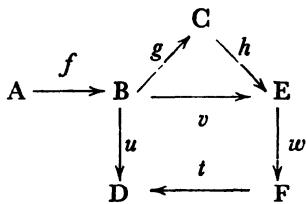
\includegraphics[keepaspectratio]{images/part003_3866b0bf02291d28d06ad2c75d3a73e7be589c55410c746bfd40818492cdc992.jpg}}

in which the letter attached to an arrow denotes a mapping of the set at the tail of the arrow into the set at its head.

The relation of equality ``f=g'' between mappings of E into F is equivalent to the relation ``for all \(x \in E, f(x) = g(x)\) ''.

\begin{enumerate}
\def\labelenumi{\arabic{enumi}.}
\setcounter{enumi}{2}
\tightlist
\item
  A function, defined on a set E, which takes the same value a for every element x of E, is called a constant function on E; it is determined by the functional relation y = a.
\end{enumerate}

The mapping of E into E which associates with each element x of E this same element is called the identity mapping. It is determined by the functional relation y = x.

If A is any subset of E, the mapping of A into E which associates with each element x of A the same element x considered as an element of E is called the canonical mapping of A into E.

Let \(f\) be a mapping of a set \(\mathbf{E}\) into itself. An element \(x\) of \(\mathbf{E}\) is said to be fixed (or invariant) under \(f\) if \(f(x) = x\) .

An element x of E is said to be fixed (or invariant) under a set of mappings of E into E if it is fixed under each of them.

\begin{enumerate}
\def\labelenumi{\arabic{enumi}.}
\setcounter{enumi}{3}
\tightlist
\item
  Let \(f\) be a mapping of \(\mathbf{E}\) into \(\mathbf{F}\) and let \(\mathbf{X}\) be any subset of \(\mathbf{E}\) . Then the image of \(\mathbf{X}\) under \(f\) is the subset \(\mathbf{Y}\) of \(\mathbf{F}\) consisting of all elements \(y\) which have the property ``there exists \(x \in \mathbf{E}\) such that \(x \in \mathbf{X}\) and \(f(x) = y\)''.
\end{enumerate}

This defines a relation between X and Y which is functional in Y and therefore determines a mapping of \(\mathfrak{P}(\mathbf{E})\) into \(\mathfrak{P}(\mathbf{F})\) . This mapping is called the canonical extension of f to sets of subsets; by abuse of language it, too, is denoted by f, and we write \(\mathbf{Y}=f(\mathbf{X})\) .

For all \(f\) and \(x\) we have

\[
f (\phi) = \phi \quad \text { and } \quad f (\{x \}) = \{f (x) \}.
\]

By abuse of language, the value \(f(x)\) of \(f\) at \(x\) is also called the image of \(x\) under \(f\) .

If y is a generic element of F, the property `` \(y \in f(E)\) '' may be expressed by saying that ``y is of the form \(f(x)\) ''.

By abuse of language, the image \(f(\mathbf{E})\) of \(\mathbf{E}\) under \(f\) is sometimes called the image of \(f\) .

If we have \(f(\mathbf{E}) = \mathbf{F}\) , that is if for all \(y \in \mathbf{F}\) there exists \(x \in \mathbf{E}\) such that \(y = f(x)\) , then \(f\) is said to be a mapping of \(\mathbf{E}\) onto \(\mathbf{F}\) , or a surjective mapping, or a surjection.

Let \(x\) be any element and \(X\) any subset of \(E\) . Instead of saying that \(f(x)\) is the value of \(f\) at \(x\) , and \(f(X)\) the image of \(X\) under \(f\) , it is sometimes said that \(f\) transforms (or maps) \(x\) into \(f(x)\) and \(X\) into \(f(X)\) ; \(f(x)\) and \(f(X)\) are then called the transforms by \(f\) of \(x\) and \(X\) , respectively.

If f is a mapping of E into itself, a subset X of E is said to be stable under f if \(f(\mathbf{X}) \subset \mathbf{X}\) . The subset X is said to be stable under a set of mappings of E into E if X is stable under each of these mappings.

\begin{enumerate}
\def\labelenumi{\arabic{enumi}.}
\setcounter{enumi}{4}
\tightlist
\item
  Let \(f\) be a mapping of \(\mathbf{E}\) into \(\mathbf{F}\) . Then we have the following propositions, in which \(\mathbf{X}\) and \(\mathbf{Y}\) denote arbitrary subsets of \(\mathbf{E}\) :
\end{enumerate}

\begin{enumerate}
\def\labelenumi{(\alph{enumi})}
\item
  The relation \(\mathbf{X} \subset \mathbf{Y}\) implies \(f(\mathbf{X}) \subset f(\mathbf{Y})\) .
\item
  The property \(\mathbf{X} \neq \emptyset\) is equivalent to \(f(\mathbf{X}) \neq \emptyset\) .
\item
  For all \(\tilde{\mathbf{X}}\) , \(\mathbf{Y}\) we have
\end{enumerate}

\begin{enumerate}
\def\labelenumi{(\arabic{enumi})}
\setcounter{enumi}{10}
\tightlist
\item
\end{enumerate}

\[
f (\mathbf {X} \cup \mathbf {Y}) = f (\mathbf {X}) \cup f (\mathbf {Y}),\tag{12}
\]

\[
f (\mathbf {X} \cap \mathbf {Y}) \subset f (\mathbf {X}) \cap f (\mathbf {Y}).
\]

\begin{enumerate}
\def\labelenumi{\arabic{enumi}.}
\setcounter{enumi}{5}
\tightlist
\item
  Let \(f\) be a mapping of \(\mathbf{E}\) into \(\mathbf{F}\) , and let \(\mathbf{Y}\) be any subset of \(\mathbf{F}\) . The inverse image of \(\mathbf{Y}\) under \(f\) is the subset \(\mathbf{X}\) of \(\mathbf{E}\) consisting of all elements \(x\) which have the property \(f(x) \in \mathbf{Y}\) .
\end{enumerate}

This defines a relation between X and Y which is functional in X and therefore determines a mapping of \(\mathfrak{P}(\mathbf{F})\) into \(\mathfrak{P}(\mathbf{E})\) , called the inverse extension of f to sets of subsets, and denoted by \(\overline{f}^{1}\) ; thus we write \(\mathbf{X} = \overline{f}^{1}(\mathbf{Y})\) .

In particular, if \(y\) is an element of \(F\) , then \(f^{1}(\{y\})\) will be the set of all \(x \in E\) such that \(f(x) = y\) . The relations `` \(f(x) = y\) '' and `` \(x \in \overline{f}^{1}(\{y\})\) '' are equivalent. By abuse of language we often write \(\overline{f}^{1}(y)\) in place of \(\overline{f}^{1}(\{y\})\) .

The trace \(X_{A}\) of a subset X of E on a given subset A is the inverse image of X under the canonical mapping of A into E (no. 3).

\begin{enumerate}
\def\labelenumi{\arabic{enumi}.}
\setcounter{enumi}{6}
\tightlist
\item
  Let \(f\) be a mapping of \(\mathbf{E}\) into \(\mathbf{F}\) . Then we have the following propositions, in which \(\mathbf{X}\) and \(\mathbf{Y}\) denote arbitrary subsets of \(\mathbf{F}\) :
\end{enumerate}

\begin{enumerate}
\def\labelenumi{(\alph{enumi})}
\item
  The relation \(\mathbf{X} \subset \mathbf{Y}\) implies \(\overline{f}^1(\mathbf{X}) \subset \overline{f}^1(\mathbf{Y})\) .
\item
  For all X, Y we have
\end{enumerate}

\begin{enumerate}
\def\labelenumi{(\arabic{enumi})}
\setcounter{enumi}{12}
\tightlist
\item
\end{enumerate}

\[
\overline {{f}} ^ {1} (\mathrm{X} \cup \mathrm{Y}) = \overline {{f}} ^ {1} (\mathrm{X}) \cup \overline {{f}} ^ {1} (\mathrm{Y}),\tag{14}
\]

\[
\bar {f} ^ {1} (\mathrm{X} \cap \mathrm{Y}) = \bar {f} ^ {1} (\mathrm{X}) \cap \bar {f} ^ {1} (\mathrm{Y}),\tag{15}
\]

\[
\overline {{f}} ^ {1} (\mathbb {C X}) = \mathbb {C} \overline {{f}} ^ {1} (\mathbf {X}).
\]

Note the difference between formulae (12) and (14); (14) would not be true for all X and Y if we replaced f by an arbitrary mapping of F into E. Again, there is no analogue of (15) for the extension of an arbitrary mapping.

Furthermore, we have \(\overline{f}^{1}(\phi) = \phi\) ; but we can also have \(\overline{f}^{1}(\mathbf{X}) = \phi\) for a non-empty subset \(\mathbf{X}\) of \(\mathbf{F}\) . In order that \(\mathbf{X} \neq \phi\) should imply \(\overline{f}^{1}(\mathbf{X}) \neq \phi\) , it is necessary and sufficient that \(f\) should be a mapping of \(\mathbf{E}\) onto \(\mathbf{F}\) .

\begin{enumerate}
\def\labelenumi{\arabic{enumi}.}
\setcounter{enumi}{7}
\tightlist
\item
  If a mapping \(f\) of \(\mathbf{E}\) into \(\mathbf{F}\) is such that for all \(y \in \mathbf{F}\) there exists at most one \(x \in \mathbf{E}\) such that \(y = f(x)\) (in other words, the set \(\overline{f}^1(y)\) is either empty or consists of a single element), then \(f\) is said to be a one-to-one mapping of \(\mathbf{E}\) into \(\mathbf{F}\) , or an injective mapping, or an injection. We have then, for all subsets \(\mathbf{X}, \mathbf{Y}\) of \(\mathbf{E}\) ,
\end{enumerate}

\[
f (\mathbf {X} \cap \mathbf {Y}) = f (\mathbf {X}) \cap f (\mathbf {Y}).\tag{16}
\]

\begin{enumerate}
\def\labelenumi{\arabic{enumi}.}
\setcounter{enumi}{8}
\tightlist
\item
  If a mapping \(f\) of \(\mathbf{E}\) into \(\mathbf{F}\) is such that for all \(y \in \mathbf{F}\) there exists exactly one \(x \in \mathbf{E}\) such that \(y = f(x)\) (in other words, \(\overline{f}(y)\) consists of a single element), then \(f\) is said to be a one-to-one mapping of \(\mathbf{E}\) onto \(\mathbf{F}\) , or a bijective mapping, or a bijection. Such a mapping may be characterized as being both a mapping of E onto F and a one-to-one mapping of E into F.
\end{enumerate}

If \(f\) is a one-to-one mapping of \(\mathbf{E}\) onto \(\mathbf{F}\) , the relation \(y = f(x)\) is not only functional in \(y\) , but also functional in \(x\) . As a functional relation in \(x\) , it determines a one-to-one mapping of \(\mathbf{F}\) onto \(\mathbf{E}\) , called the inverse of the mapping \(f\) .

Note that the extension of the inverse of f is the same as the inverse of the extension of f.

Let \(g\) be the inverse of \(f\) . Then the relations `` \(y = f(x)\) '' and `` \(x = g(y)\) '' are equivalent. The inverse of \(g\) is \(f\) . If \(f\) is a one-to-one mapping of \(E\) onto \(F\) , we have not only the relation (16) but also, for all subsets \(X\) of \(E\) ,

\[
f (\mathbf {C X}) = \mathbf {C} f (\mathbf {X}).
\]

Moreover, the extension of \(f\) is a one-to-one mapping of \(\mathfrak{P}(\mathbf{E})\) onto \(\mathfrak{P}(\mathbf{F})\) .

A one-to-one mapping of E onto F, together with its inverse mapping, are said to realize a one-to-one correspondence between E and F; alternatively, we say that E and F are put in one-to-one correspondence by these mappings.

A one-to-one mapping of a set E onto itself is called a permutation of E. The identity mapping is a permutation. If a permutation is identical with its inverse, it is said to be involutory; for example, the mapping \(X \rightarrow C X\) of \(\mathfrak{P}(E)\) onto itself is involutory.

\begin{enumerate}
\def\labelenumi{\arabic{enumi}.}
\setcounter{enumi}{9}
\tightlist
\item
  In the following propositions, X denotes an arbitrary subset of E, and Y an arbitrary subset of F :
\end{enumerate}

\begin{enumerate}
\def\labelenumi{(\alph{enumi})}
\tightlist
\item
  If \(f\) is a mapping of \(\mathbf{E}\) into \(\mathbf{F}\) , we have
\end{enumerate}

\begin{enumerate}
\def\labelenumi{(\arabic{enumi})}
\setcounter{enumi}{16}
\tightlist
\item
\end{enumerate}

\[
\overline {{{f}}} ^ {1} (\mathrm{Y}) = \overline {{{f}}} ^ {1} (\mathrm{Y} \cap f (\mathrm{E})),\tag{18}
\]

\[
\mathbf {X} \subset \overline {{f}} ^ {1} (f (\mathbf {X})),\tag{19}
\]

\[
f (\overline {{f}} ^ {1} (\mathbf {Y})) \subset \mathbf {Y}.
\]

\begin{enumerate}
\def\labelenumi{(\alph{enumi})}
\setcounter{enumi}{1}
\item
  The properties ``for all Y, \(f(\bar{f}^{1}(Y)) = Y\) '' and ``f is a mapping of E onto F'' are equivalent.
\item
  The properties ``for all X, \(\overline{f}^{1}(f(X)) = X\) '' and ``f is a one-to-one mapping of E into F'' are equivalent.
\item
  The properties ``for all X and Y,
\end{enumerate}

\[
\bar {f} ^ {1} (f (\mathbf {X})) = \mathbf {X} \quad \text { and } \quad f (\bar {f} ^ {1} (\mathbf {Y})) = \mathbf {Y}"
\]

and ``f is a one-to-one mapping of E onto F'' are equivalent.

\begin{enumerate}
\def\labelenumi{\arabic{enumi}.}
\setcounter{enumi}{10}
\tightlist
\item
  Let E, F, G be three sets, which may or may not be distinct. Let f be a mapping of E into F, and let g be a mapping of F into G. The mapping of E into G whose value at any element x of E is \(g(f(x))\) is called the composition of g and f, and is denoted by \(g \circ f\) , or simply gf if there is no risk of ambiguity.
\end{enumerate}

The equality \(h = g \circ f\) is called a factorization of h.

Note that, if G is distinct from E, we may not speak of the composition of f and g (in that order), and the notation \(f \circ g\) has no meaning. If G is identical with E, then \(f \circ g\) and \(g \circ f\) are not elements of the same set unless F is also identical with E; and even when this is so, it is usually the case that \(f \circ g \neq g \circ f\) . Thus the order of composition of f and g is essential.

Let \(\varphi\) be the composition of \(g\) and \(f\) , let \(\mathbf{X}\) be any subset of \(\mathbf{E}\) , and let \(\mathbf{Z}\) be any subset of \(\mathbf{G}\) . Then we have

\begin{enumerate}
\def\labelenumi{(\arabic{enumi})}
\setcounter{enumi}{19}
\tightlist
\item
\end{enumerate}

\[
\varphi (\mathbf {X}) = g (f (\mathbf {X})),\tag{21}
\]

\[
\overline {{{\varphi}}} ^ {1} (Z) = \overline {{{f}}} ^ {1} (\overline {{{g}}} ^ {1} (Z)).
\]

If \(f\) is a one-to-one mapping of \(\mathbf{E}\) onto \(\mathbf{F}\) , and if \(g\) is a one-to-one mapping of \(\mathbf{F}\) onto \(\mathbf{G}\) , then \(g \circ f\) is a one-to-one mapping of \(\mathbf{E}\) onto \(\mathbf{G}\) .

Let \(h\) be a mapping of \(G\) into a set \(H\) . Then we have

\[
h \circ (g \circ f) = (h \circ g) \circ f;
\]

this mapping of E into H is written \(h \circ g \circ f\) , and is called the composition of the three mappings h, g, f in this order. The composition of more than three mappings is defined similarly.

If \(f\) is a mapping of \(\mathbf{E}\) into itself, the iterates of \(f\) are defined to be the mappings \(f^n\) ( \(n\) an integer \(\geqslant 1\) ) of \(\mathbf{E}\) into itself, defined by induction on \(n\) by means of the relations \(f^1 = f\) , \(f^n = f^{n-1} \circ f\) ; \(f^n\) is called the nth iterate of \(f\) . We have \(f^{m+n} = f^m \circ f^n\) .

\begin{enumerate}
\def\labelenumi{\arabic{enumi}.}
\setcounter{enumi}{11}
\tightlist
\item
  In general, the composition \(\overline{f}^{1} \circ f\) of the inverse extension and the extension of a mapping \(f\) is not the identity mapping of \(\mathfrak{P}(\mathbf{E})\) onto itself. Likewise, \(f \circ \overline{f}^1\) is not usually the identity mapping of \(\mathfrak{P}(\mathbf{E})\) onto itself. These two conditions are satisfied simultaneously only if \(f\) is a bijection of \(\mathbf{E}\) onto \(\mathbf{F}\) .
\end{enumerate}

If \(f\) is a bijection of \(\mathbf{E}\) onto \(\mathbf{F}\) , and if \(g\) denotes the inverse of \(f\) , then the compositions \(g \circ f\) and \(f \circ g\) are respectively the identity mapping of \(\mathbf{E}\) onto \(\mathbf{E}\) and the identity mapping of \(\mathbf{F}\) onto \(\mathbf{F}\) .

Conversely, if \(f\) is a mapping of \(\mathbf{E}\) into \(\mathbf{F}\) , and \(g\) a mapping of \(\mathbf{F}\) into \(\mathbf{E}\) , such that \(g \circ f\) is a permutation of \(\mathbf{E}\) and \(f \circ g\) is a permutation of \(\mathbf{F}\) , then \(f\) is a bijection of \(\mathbf{E}\) onto \(\mathbf{F}\) and \(g\) is a bijection of \(\mathbf{F}\) onto \(\mathbf{E}\) .

If, moreover, \(g \circ f\) is the identity mapping of \(\mathbf{E}\) onto itself, then \(g\) is the inverse of \(f\) .

\begin{enumerate}
\def\labelenumi{\arabic{enumi}.}
\setcounter{enumi}{12}
\item
  Let \(f\) be a mapping of \(\mathbf{E}\) into \(\mathbf{F}\) , and let \(\mathbf{A}\) be any subset of \(\mathbf{E}\) . The mapping \(f_{\mathbf{A}}\) of \(\mathbf{A}\) into \(\mathbf{F}\) whose value at any element \(x\) of \(\mathbf{A}\) is \(f(x)\) is called the restriction of \(f\) to the subset \(\mathbf{A}\) ; it is just the composition of \(f\) and the canonical mapping of \(\mathbf{A}\) into \(\mathbf{E}\) . If two mappings \(f, g\) of \(\mathbf{E}\) into \(\mathbf{F}\) have the same restriction to \(\mathbf{A}\) , they are said to agree (or coincide) on \(\mathbf{A}\) . Conversely, \(f\) is said to be an extension of \(f_{\mathbf{A}}\) to \(\mathbf{E}\) .
\item
  A mapping of a set E onto a set F is also called a parametric representation of F by means of E; E is then called the parameter set of this representation, and the elements of E take the name of parameters.
\end{enumerate}

A family of elements of a set F is by definition a subset of F endowed with a parametric representation; in other words, to be given a family of elements of F is equivalent to being given a mapping of some set E into F. The image of E under this mapping is called the set of elements of the family. Note that two distinct families of elements of F may have the same subset of F as the set of their elements.

With each subset A of a set F we may always associate a family of elements whose set of elements is A. It is enough to consider the family defined by the canonical mapping of A into F.

A family of elements of F, defined by a mapping \(\iota\to x_{i}\) of a set I into F, is denoted by \((x_{i})_{i\in I}\) , or simply \((x_{i})\) if there is no possible ambiguity about the index set.

If \(J\) is a subset of \(I\) , the family \((x_{t})_{t\in J}\) is called the subfamily corresponding to \(J\) of the family \((x_{t})_{t\in I}\) ; it is defined by the restriction to \(J\) of the mapping \(t\to x_t\) .

